\newpage
\section{Comparing recursive bisection to direct k-way partitioning [10 points]}
In this exercise the goal is to compare and analyze the performance of recursive bisection and direct k-way partitioning by looking at the edge cut result. Both methods are using Metis and the goal is to partition the graphs into 16 (Table~\ref{tab:partitions_rec}) and 32 (Table~\ref{tab:partitions_k_way}) partitions. Comparing the two methods we can clearly see that that direct k-way partitioning consistently outperforms the recursive bisection by creating a smaller edge cut. This is the case because recursive bisection has no global information when doing partitioning decisions, k-way on the other hand overcomes this limitation by coarsening the graph first and the then refining the partitioning. Knowing this coarsening and refinement steps it was anticipated that k-way partitioning would outperform recursive bisection. Another observation that can be made is that the difference in edge cut between the methods increases when comparing 16 to 32 partitions. Indicating that k-way multiway partitioning also scales better in terms of number of partitions.
\begin{table}[H]
	\centering
	\begin{tabular}{lccccccc} % Note the number of columns matches the data
		\toprule
		Partitions & Luxemburg & USRoads & Greece & Switzerland & Vietnam & Norway & Russia \\
		\midrule
		16         & 191       & 585        & 318    & 685         & 270     & 271    & 572    \\
		32         & 317       & 983        & 500    & 1067        & 445     & 509    & 941    \\
		\bottomrule
	\end{tabular}
	\caption{Cut edges for recursive bisection.}
	\label{tab:partitions_rec}
\end{table}

\begin{table}[H]
	\centering
	\begin{tabular}{lccccccc} % Ensure this matches your data columns
		\toprule
		Partitions & Luxemburg & USRoads & Greece & Switzerland & Vietnam & Norway & Russia \\
		\midrule
		16         & 185       & 545        & 301    & 665         & 231     & 241    & 551    \\
		32         & 304       & 921        & 486    & 1013        & 418     & 436    & 931    \\
		\bottomrule
	\end{tabular}
	\caption{Cut edges for direct multiway partitioning in Metis 5.0.2.}
	\label{tab:partitions_k_way}
\end{table}
Figure~\ref{fig:metis} showcases how various examples of graphs are partitioned differently when using recursive or k-way partitioning.

\begin{figure}[H]
	\centering
	\begin{subfigure}{0.5\textwidth}
		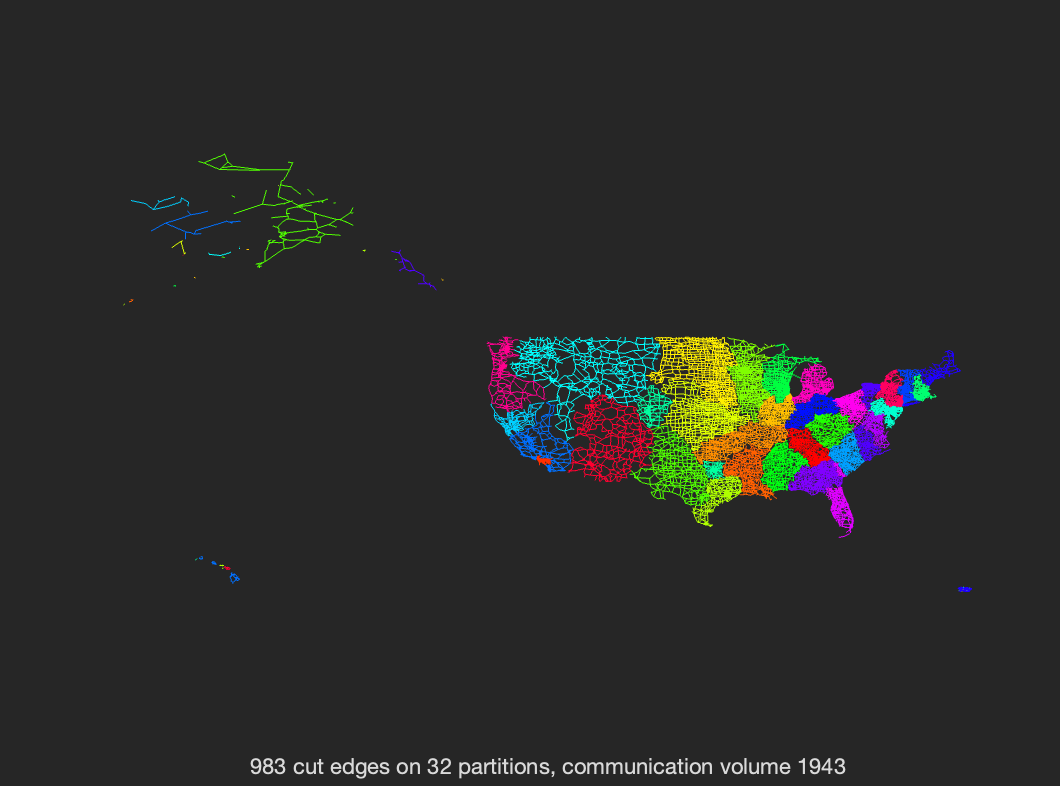
\includegraphics[width=\textwidth]{./media/usa_metis.png}
		\caption{USA with recursive bisection}
		\label{fig:usa_metis}
	\end{subfigure}%
	~
	\begin{subfigure}{0.5\textwidth}
		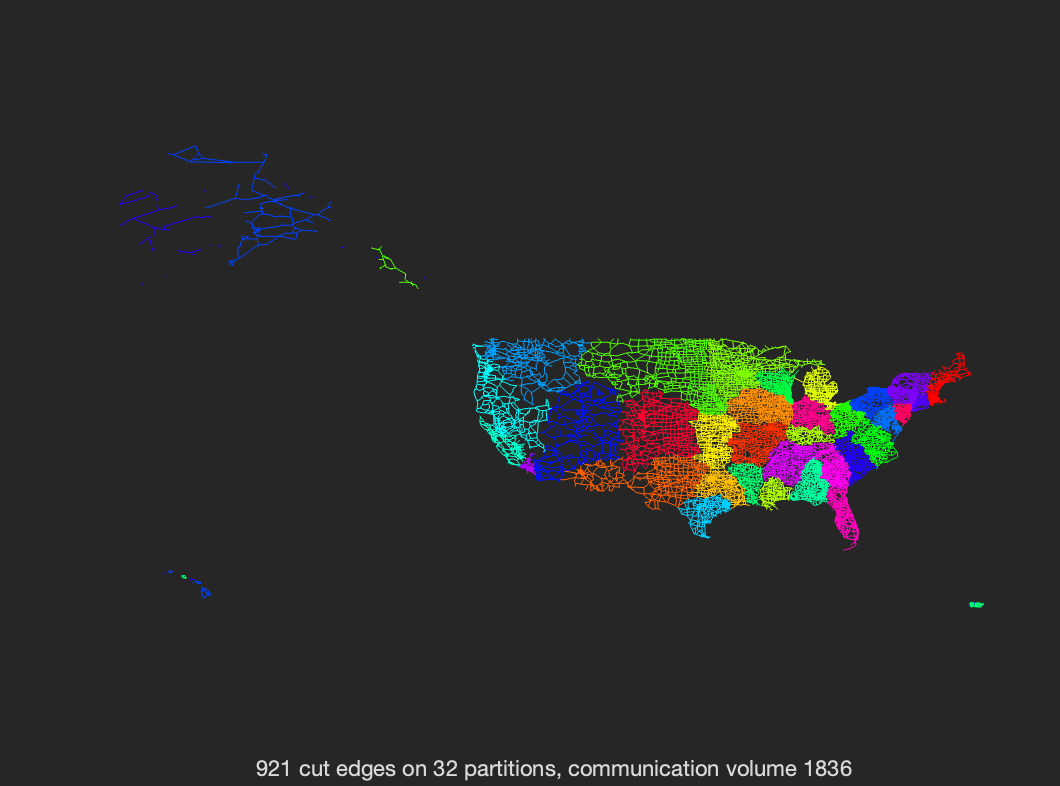
\includegraphics[width=\textwidth]{./media/usa_metis_k.png}
		\caption{USA with direct multiway partitioning}
		\label{fig:usa_metis_k}
	\end{subfigure}\\
	\begin{subfigure}{0.5\textwidth}
		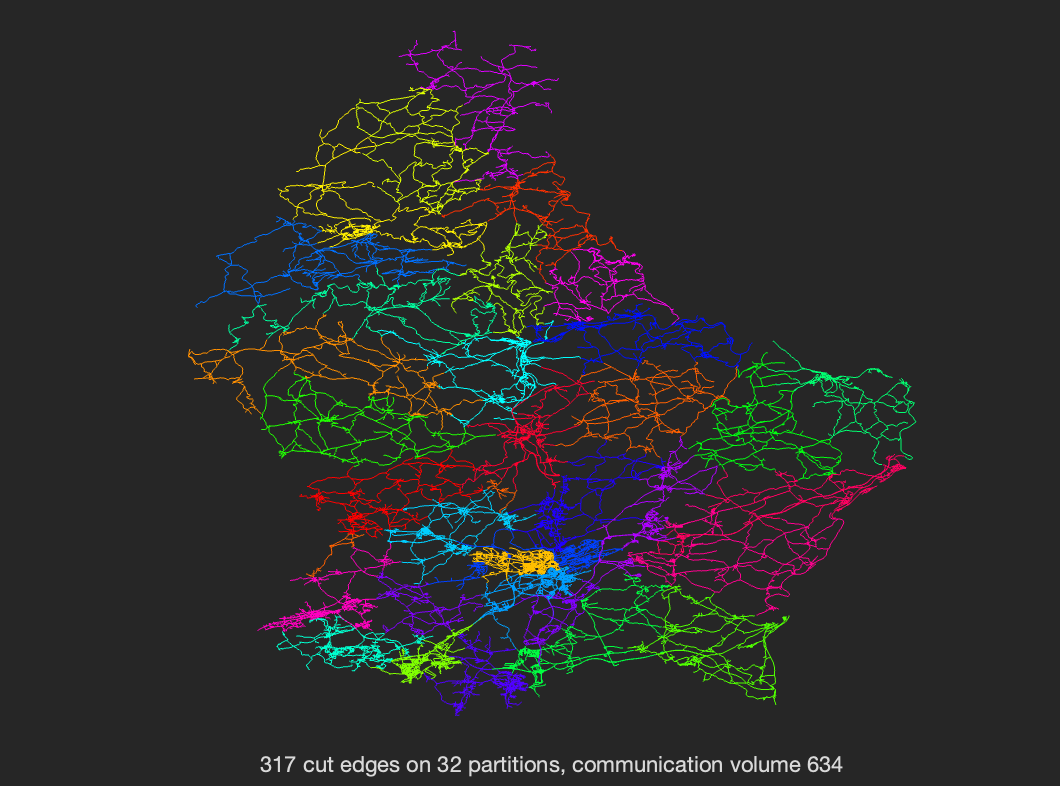
\includegraphics[width=\textwidth]{./media/lux_metis.png}
		\caption{Luxembourg with recursive bisection}
		\label{fig:lux_metis}
	\end{subfigure}%
	~
	\begin{subfigure}{0.5\textwidth}
		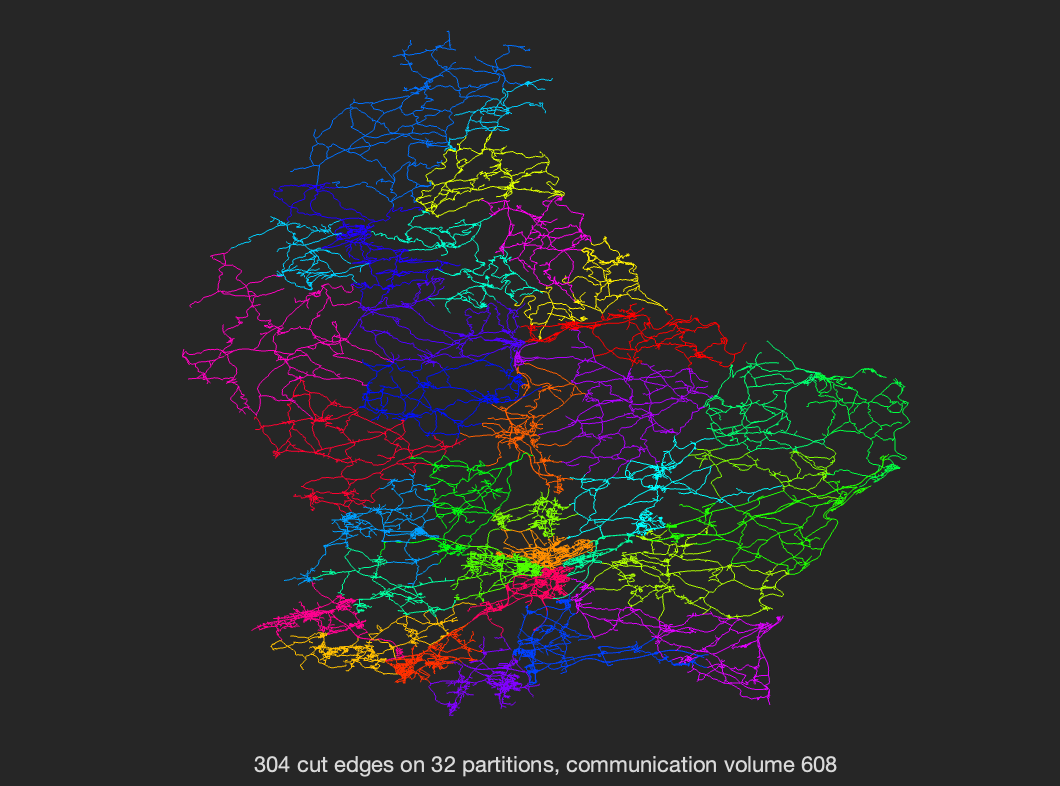
\includegraphics[width=\textwidth]{./media/lux_metis_k.png}
		\caption{Luxembourg with direct multiway partitioning}
		\label{fig:lux_metis_k}
	\end{subfigure}
	\begin{subfigure}{0.5\textwidth}
		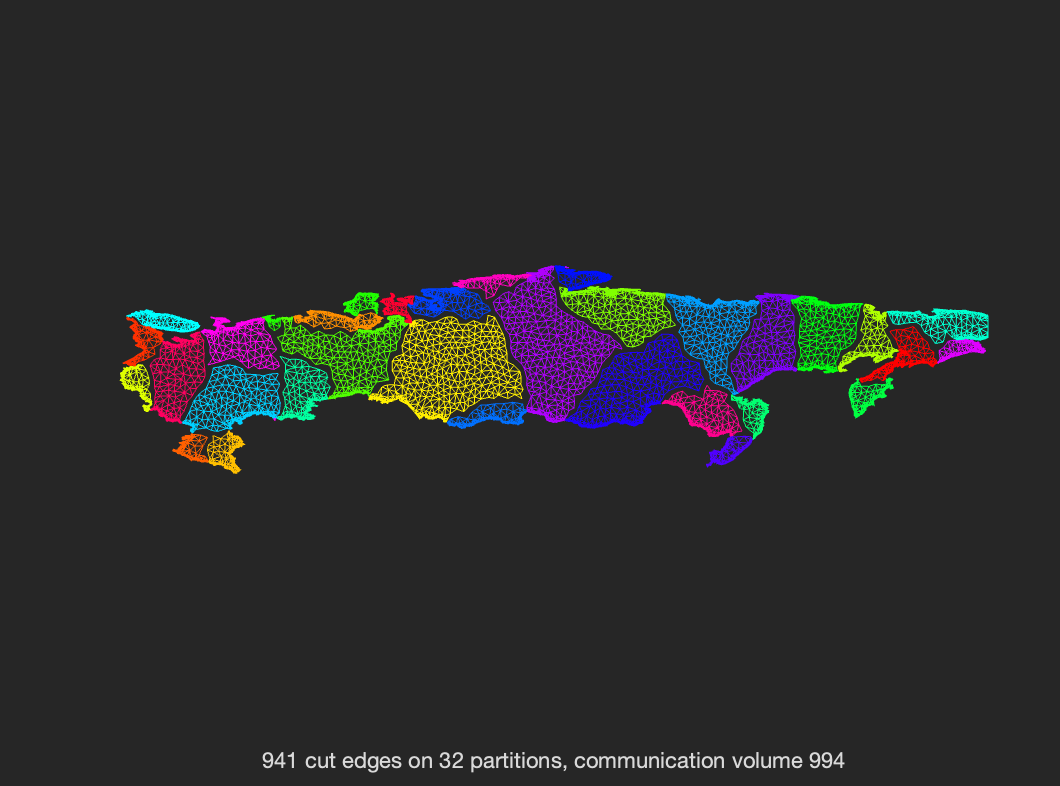
\includegraphics[width=\textwidth]{./media/ru_metis.png}
		\caption{Russia with recursive bisection}
		\label{fig:ru_metis}
	\end{subfigure}%
	~
	\begin{subfigure}{0.5\textwidth}
		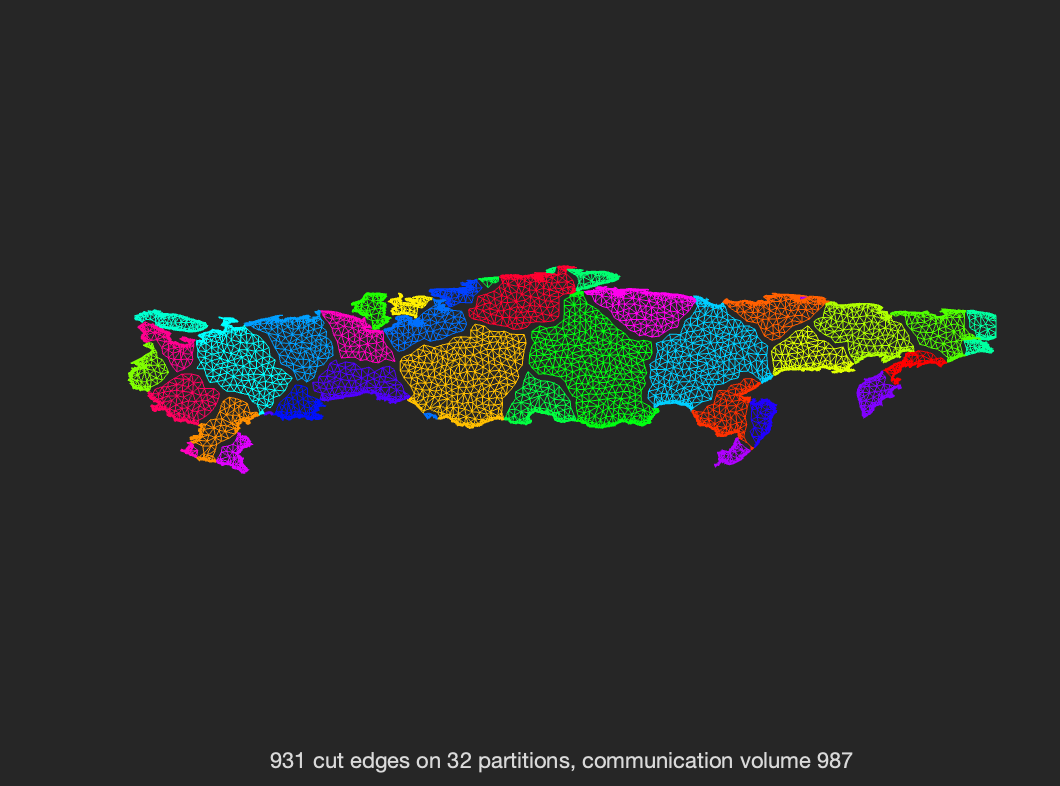
\includegraphics[width=\textwidth]{./media/ru_metis_k.png}
		\caption{Russia with direct multiway partitioning}
		\label{fig:ru_metis_k}
	\end{subfigure}

	\caption{Partitioning results for the graphs of USA, Luxemburg, and Russia
for 32 partitions}
	\label{fig:metis}
\end{figure}

